%%%%%%%%%%%%%%%%%%%%%%%%%%%%%%%%%%%%%%%%%%%%%%%%%%%%%%%%%%%%%%%%%%%%%%%%%%%%%%%%%%%%%
% Template revision history:
% BS2021: Revised by Filip Jorissen, filip.jorissen@kuleuven.be
% BS2019: Revised by Alessandro Prada, alessandro.prada@unitn.it
% BS2017: Initial version by Michael Wetter, mwetter@lbl.gov
%%%%%%%%%%%%%%%%%%%%%%%%%%%%%%%%%%%%%%%%%%%%%%%%%%%%%%%%%%%%%%%%%%%%%%%%%%%%%%%%%%%%%

\documentclass[twocolumn, a4paper,10pt]{article}
\usepackage[top=2.5cm, bottom=2.5cm, left=2.0cm, right=2.0cm,
columnsep=0.8cm]{geometry}
\usepackage{enumitem}
\usepackage[hidelinks]{hyperref}
\usepackage{boxedminipage}
\usepackage{nopageno}
\usepackage{graphicx}
\usepackage{natbib}
\usepackage[font=it]{caption}
\usepackage[usenames,dvipsnames]{xcolor}
\usepackage{listings}
\usepackage{caption}
\usepackage{subcaption}
%-----------------------------SET SKIP SPACES -------------------------------------------------------------------
\setlength{\abovecaptionskip}{0pt}
\setlength{\belowcaptionskip}{3pt}
\setlength{\parindent}{0pt}
\setlength{\parskip}{3pt}
%\renewcommand{\baselinestretch}{0.7}
% FOR enumerates
\setlist{itemsep=-0.1cm,topsep=0.1cm,labelsep=0.3cm}
\setenumerate{leftmargin=*}
\setcounter{secnumdepth}{-1}
%-----------------------------SET FONTS -------------------------------------------------------------------
% Set fonts for title, section and subsection headings
\makeatletter
\renewcommand\title[1]{\gdef\@title{\fontsize{12pt}{2pt}\bfseries{#1}}}
\makeatletter
\renewcommand\section{\@startsection{section}{1}{\z@}{3pt}{3pt}{\normalfont\large\bfseries}}
% \normalfont\large
\makeatletter
\renewcommand\subsection{\@startsection{subsection}{1}{\z@}{\z@}{\z@}{\normalfont\normalsize\bfseries}}
\makeatletter
\renewcommand\subsection{\@startsection{subsection}{1}{\z@}{\z@}{0.1pt}{\normalfont\normalsize\bfseries}}
\renewcommand\refname{References}
%END OF THE SETUP
%%%%%%%%%%%%%%%%%%%%%%%%%%%%%%%%%%%%%%%%%%%%%%%%%%%%%%%%%%%%
% Simulation and visualisation of mitigation and adaption strategy pathways for urban districts
%%%%%%%%%%%%%%%%%%%%%%%%   TITLE   %%%%%%%%%%%%%%%%%%%%%%%%%%%%%%%
%%% Please keep the \vspace{4pt} at the top
\title{%
Simulation and visualization framework for decision making of climate mitigation  																								% Line 1
%%% Please keep the \vspace{4pt} between lines in the title
\vspace{4pt}
and adaptation strategies in new and existing urban development} 																																% Line 2 
%If there is no second line then just put \phantom{Line 2} here
%%% Change or delete text before "\\" on the lines below to keep the layout but don't remove the "\\"
%%% Do not exceed more than 6 lines for authors and affiliations
\author{																																														% Line 3
% Justin McCarty$^1$, Adam Rysanek$^1$
\\ 																				% Line 4
% $^1$The University of British Columbia, Vancouver, Canada
\\ 																																                                                            	% Line 5
% $^2$Institution 2, City 2, Country 2
\\ 																																                                                                % Line 6
% comment the lines below and add \phantom{} lines as needed to reach a total of 10 lines
% \textit{(The names and affiliations SHOULD NOT be included in the draft submitted for review)}
\\ 			 			  	                                                    % Line 7
% \textit{(leave blank up to line 10 - remove line numbering from final version)}
\\ 														                    	% Line 8
\phantom{Line 9}} 																																								            	% Line 9
\date{\vspace{-0.5cm}}	% remove default date and replace the Blank 10th line														                                                            % Line 10
%END OF THE TITLE
%%%%%%%%%%%%%%%%%%%%%%%%%%%%%%%%%%%%%%%%%%%%%%%%%%%%%%%%%%%%
\begin{document}

\maketitle

\section*{Abstract}	% Section headings need to be upper and lower case.
\addtocounter{section}{1}
At present mitigation and adaptations strategies compete for constrained resources within a future of uncertain climate impacts. Meeting decarbonisation goals while implementing robust and resilient adaptions strategies requires an analysis structure that can account for uncertainty as well as depict how the intermingling of strategies may hinder or benefit the ultimate trajectory of actions. The marginal abatement cost curve (MACC) is an indispensable tool for planning mitigation pathways, but has historically not relied upon robust experimental analysis making it notional at best nor has it included a view of adaptation pathways. This study utilizes a recently developed and nearly finished medium-density community in Vancouver, British Columbia, Canada of 15,000 residents as a case study for developing a pathway based MACC. Multiple mitigation and adaptation measures are modeled individually and through exhaustive combination to test their sensitivity on marginal abatement cost and residual cost of climate change. The resulting MACCs are compared with more tradition decision support visualizations to argue for a more comprehensive approach to decarbonisation and adaptation planning. 

\section*{Key Innovations}
\begin{itemize}
\item Visualization of marginal abatement cost of urban scale building and energy system interventions.
\item Intermingling of climate change mitigation and adaptation strategies in a decision making framework for development planning.
\item The inclusion of embodied carbon as a metric in determining carbon emissions and marginal abatement cost.
\end{itemize}

\section*{Practical Implications}
Open-source simulation tools can be used to test the sensitivity of different decarbonisation and adaptation strategies for an urban area, allowing planners better models to make planning decisions. 

%---------------------------------------------------------------------------------------
\section*{Introduction}

Atmospheric concentrations of carbon dioxide lie northward of 410 parts per million, while recent estimates from the \citet{ncdc} situate the Northern Hemisphere’s land and ocean surface temperature anomaly at 1.29°C from baseline (1961-1990). This may not be considered a consistent level of \textit{global warming}, but it does point the dangerous warming trend facing human and non-human systems. Due to the cumulative warming of the planet, climate change impacts are now being recognized as burdens on economic and social systems [X attribution science report for 2020]. Implementing adaptation strategies within the built environment is necessary to increase social resilience, protect safety and life, and prevent economic damage with the potential to bolster all of the above [X cobenefits of adaptation paper]. Simultaneously, the mitigation of present emissions, the abatement of possible future emissions, and the sequestration of atmospheric carbon is necessary to curtail increasingly dangerous and catastrophic levels of warming. This process of carbon drawdown is very familiar within studies of the built environment with strategies posed for transportation, buildings, agriculture, forestry, and other landuses. Mitigation and adaptation strategies though are rarely evaluated simultaneously in the context of urban development.

In the presence of limited resources and a range of objectives, the cost and benefit of proposed strategies need to be assessed on their own and while interacting with other strategies, as well as under the uncertainty of climate change and human action. The interaction of strategies is a key factor explored in \citet{rysanek MACC}, where exhaustive simulation of the possible strategies, depicted in Figure \ref{fig:sample_sequence}, is applied in the modeling of fifteen individual building retrofit strategies (a total of 32,768 unique combinations). From this database of simulated retrofits specific pathways for building retrofit can be generated. However, \citet{rysanek MACC} note that this process may not be desirable for every retrofit project that concerns only one building as the overhead cost of developing such a model is large and requires extensive computing resources. However, in the application of urban retrofit modeling for the purposes of enhancing policy making and incentive creation this framework could prove useful.

Introducing the scale of a neighborhood or even entire city affords the use of an extensive modelling framework as described above, but further uncertainty is encountered in this problem space when considering urban development. No longer is the model concerned with answering a single question about a single existing building - how do we mitigate the most carbon at the lowest price? Now, the model is being applied in the context of an existing area where buildings and empty plots face a \textit{known-unknown} trajectory of new development, redevelopment, and no change. This brings in a the concept of a development timeline during which differing scales of development may occur.

The resulting simulation database can be used to assess decarbonization pathways that align with development trajectories and/or different degrees of global warming. The difficulty though is in interpreting a large quantity of simulation data for its salience in the decarbonization and adaptation space. Several (\citep{various MACC papers}) have proposed marginal abatement cost curves (MACCs) as a useful metric to compare strategies, while \citet{kesicki} points out that their use should be tempered with caution related to the lack of interaction of strategies in typical MACCs, a point countered by \citet{rysanek MACC} through an underlying sequential and exhaustive simulation framework. Applying this same framework to the task of determining optimal decarbonization pathways through mitigation strategies can result in a viable set of MACCs for planing and policy support.

The literature on MACCs has not yet involved adaptation strategies as a form of emissions mitigation. However, as noted earlier adaptation and mitigation strategies ,may be decide upon fro the same funding perspective and therefore need to be considered together. Therefore this study integrates several adaptations strategies into the simulation process. These adaptation strategies are evaluated on the basis of marginal abatement cost, as well as their influence on the adaptation of the the development. Therefore mitigation strategies are equally evaluated as adaptations strategies. 

This study will test the performance of adaptation and mitigation strategies alongside one development pathway and two climate change pathways, simulated at two points in time (2050 and 2080), for a case study community in southwestern Canada; Wesbrook Village, Vancouver, British Columbia (BC). A baseline urban building energy model (UBEM) was created to represent the development of the community to-date, shown in Figure \ref{fig:wesbrook_base} alongside the future development and climate change pathways.

\begin{figure}
    \centering
    \includegraphics{}
    \caption{A sample of how }
    \label{fig:sample_sequence}
\end{figure}

\begin{figure}
    \centering
    \includegraphics{}
    \caption{The baseline UBEM for Wesbrook Village in BC.}
    \label{fig:wesbrook_base}
\end{figure}

\subsection*{Wesbrook Village} 
Simulation will be exhaustive of the different combinations in the pool of strategies and scenarios allowing each strategy to be measured independently as well as determine combinations that are more or less efficient than individual implementation under the entire range of uncertainty.

Wesbrook Village and the neighbouring Stadium Road are new communities that expected to reach 715,925 sqm. of residential floor space and 10,000 sqm. of non-residential floor space by 2040. It is the part of a larger community plan led by the development arm of The University of British Columbia (UBC) \citep{wesbrook plan; stadium plan}. The baseline for this study is taken at the end of 2020, where the development has completed its fifteenth year. The development, referred to throughout the study as \textit{Wesbrook}, is a compelling case study as it can be considered a model of medium-density new development for BC and North America at large. Building code for the community is modeled after the aspirational provincial code made more strict through a continuous review with the most recent version taking effect in January 2021 and targeting net-zero energy ready (NZER) by 2032; NZER buildings are built such that with the addition of solar panels or renewable technologies they would consume only as much energy as they produce. The energy system is a mixture of grid-connected systems, in building natural gas boilers, and a district heating system that supplies hydronic baseboard and floor heating systems as well as domestic hot water. This district heating system, described in \citet{McCarty 2021}, is designed to migrate from natural gas boilers to heat pumps fed by waste heat from a nearby particle accelerator facility that is trimmed up by peaking natural gas boilers. Cooling services have yet to considered in spec-residential development in BC as the climate has historically allowed comfort to be achieved in the peak of summer through natural ventilation; research however indicates that this is quickly becoming an obsolete design standard due to climate change \citep{ML cooling paper}. The intention with the code development for this community will however require cooling in buildings soon.  

\subsubsection*{Retrofit and New Development Trajectory}
The majority of Wesbrook has been completed as of 2020, with 50\% of the total expected build-out of 725,925 sqm. remaining between now and the mid-21st century. As indicated in Figure \ref{fig:wesbrook_base} the yet-to-be-completed development will be assessed in the model through the future periods. While in less centrally planned and developed communities tackling development uncertainty would require a more thorough economic model, the Wesbrook planning and development scheme is well laid out in master-planning documents \citep{Wesbrook masterplan}. The simulation framework is built from a baseline in 2020 of the completed development up to 2020. Two more time periods were simulated, the first in 2050 and then in 2080. The base-case for each time period assumes that the stock of buildings that were simulated in the previous time-step (existing) were retrofitted with similarly performing technologies and components. New buildings are however built to a performance profile modeled after the code trajectory referenced in Table \ref{tab:code_trajectory}. While it is expected that the future will hold more advanced technologies, code development is capped at the introduction of the NZER requirements.

\begin{table*}[h]
    \vspace{-5pt}   % Please use appropriate negative vspace to remove the space above/belovw the Table
    \caption{The first two-column table.}
    \label{tab:code_trajectory}
    \centering
    \begin{tabular}{ | c | c | c | }
        \hline
        \bf{Heading 1} & \bf{Heading} 2 & \bf{Heading 3} \\
        \hline
        Entry 1 & Entry 2 & Entry 3 \\
        \hline
    \end{tabular}
    \vspace{-5pt}   % Please use appropriate negative vspace to remove the space above/belovw the Table
\end{table*}

\subsection*{Mitigation and adaptation decision tools}
\citet{Rysanek MACC} expanded on the use of marginal abatement cost curves as a tool for planning retrofit pathways in single building optimization. The authors commentary was that by failing to consider technical and economic interactions MACCs such as those proposed by \citet{Mckinnsey} were inauthentic. Without accounting for the additionality of measures many MACCs fall into this grouping and limit their overall effectiveness. \citet{kesicki} acknowledges temporal interactions as an additional dimension that need to be considered when constructing MACCs. Traditionally MACCs were developed for annual-planning and more recently, as ambition has grown, so too have their temporal scales. These interactions can be summarized as understanding how investments made in the past may affect the outcome of the MACC, similar to the issue of technical and economic interactions. In planning buildings or infrastructure with MACCs this becomes a significant feature to consider as selecting investments to implement, one typically does so along an investment pathway. 

It is also of particular importance when developing infrastructure or buildings to consider the impact of a changing climate. Adaptation is prevalent in designing buildings in proximity to rising seas, adaptation ranges from hard to soft measures such as levies and dams to wetland restoration \citep{IPCC WGIIAR5 CH 15}. Evidence is pointing to the need to consider other impacts, such as overheating risk due to generally warmer days, nights with less cooling capacity, and more intense heat waves \citep{Lomas and Porrit; Rysanek ML Paper}. Measuring adaptation is a contentious field, as what defines successful adaptation is not as simple to calculate as net carbon emissions \citep{IPCC WGIIAR5 CH 14}. \citet{Brooks et al.} suggests several general criteria by which successful adaptation can be assessed: feasibility, efficacy/effectiveness, efficiency, acceptability/legitimacy, equity, and sustainability. The same authors also discuss the concept of Maladaptation, or the inadvertent increase in vulnerability to climate change as a result of development, which has equal importance to adaptation planning of buildings. For all criteria though, measures begin with assessing vulnerability of a subject to a stressor or collection of stressors. In the case of coastal development, a building's adaptive capacity and success can be measured by its vulnerability to increasingly intense sea level rise and storm surge. In the case of this study the stressor is heat gain and the vulnerability of a building to overheating. 

Metrics to evaluate adaptive capacity and ultimate effectiveness of measures are not concrete, as the metric typically has to be defined for the problem space \citep{brooks 2011}. 


%---------------------------------------------------------------------------------------
\section*{Methods}

\subsection*{Urban Building Energy Model}
The simulation framework utilizes an extension of the City Energy Analyst (CEA) demand forecasting model \citep{CEA, Fonseca1, Fonseca2}. The CEA enables simulations of urban and neighborhood scale energy systems, as well as independently operating buildings. It is a hybrid dynamic statistical model that allows for efficient processing times, a necessity for large simulation sets such as the one in this study.

The urban building energy model (UBEM) consists of a base-case of development and two future states of development, one in 2050 and another in 2080. The base-case was simulated once to tune the model. Each of the future states of development were simulated once for each combination of strategies under both climate change scenarios for a total of 1024 simulations.  

The UBEMs are low-level of detail geometrically described by their heights above and below ground, window to wall ratio, and composition of envelope, HVAC, and energy supply traits, described in full in Table \ref{tab:model_parameters}. 

\begin{table}[ht]
    \vspace{-5pt}   % Please use appropriate negative vspace to remove the space above/belovw the Table
    \caption{Example of a table.}
    \label{tab:model_parameters}
    \centering
    \begin{tabular}{| c | c | c | }
        \hline
        \bf{Heading 1} & \bf{Heading} 2 & \bf{Heading 3} \\
        \hline
        Entry 1 & Entry 2 & Entry 3 \\
        \hline
    \end{tabular}
    \vspace{-5pt}   % Please use appropriate negative vspace to remove the space above/belovw the Table
\end{table}

\subsection*{Boundary conditions}
The EnergyPlus Weather (EPW) file for Vancouver, BC produced by \citet{CWEC 2016 citation} was morphed, following the algorithms set out by \citet{Belcher} and expanded upon by \citet{CCworldweathergen}. These methods utilize the monthly delta of a region's between historical climate models and a projected pathway \citep{SSPs} to adjust the hourly values contained in an EPW file. Variations on the morphing process have been found, accounting for different shortcomings or the availability of more resolute climate model data to describe a region's specific topographic or climatic uniqueness that may not be captured in a typical climate model's often 100km x 100km grid.

The morphing process in this study differs from previous examples in that it was able to make use of the latest generation of global climate models \citep{CMIP6 text}. The morphing process took into account an ensemble of 24 models for calculating projected hourly temperature, solar radiation, cloud cover, relative humidity, wind speed, and air pressure. Morphed variables and ensemble composition is described in Table \ref{tab:model_table} The morphing process produced four morphed EPWs from two climate change pathways at two time periods, described in Figure \ref{fig:weatherfiles}.

\subsection*{Strategies}
Eight mitigation and adaptation strategies were selected to evaluate under the development pathways and climate change pathways. The strategies, show in Table \ref{tab:strategies}, reflect larger interventions into either existing buildings, new buildings, both, or the underlying energy system in the community. A strategy is implemented alone as well as in combination with the other seven to understand its range of potential impacts, which assists the decision-making framework in determining a pathway to implement strategies.

\subsection*{Simulation}
For each development period and under each climate change pathway the same eight strategies for decarbonization and adaptation to a changing climate were evaluated for their marginal cost of carbon abatement across the whole the Wesbrook development Strategies were tested on their own and in an exhaustive combination with the other seven strategies. The simulation procedure for each scenario began with the base-case, under which no strategies were implemented, following with 255 iterations where strategies where implemented alone and in combination with each other. This was repeated across both development pathways and both climate change pathways, leading to 1024 iterations of the model. The advantage of the underlying simulation technology, CEA, is that demand forecasting can be performed parallelized through multithreading, greatly improving processing time at three minutes per iteration \citep{multithreading package}. At the time of writing radiation analysis was not able to be brought out of a single CPU core and thus steps were taken to minimize the amount of times the command was used as the processing time for the ~120 buildings in the UBEM was 25 minutes. In each scenario only 16 experiments required unique radiation profiles. These were run first in the loop of 256. The 240 simulations that followed then copied the appropriate output files from the radiation analysis. District heating primary energy requirement was modeled post-simulation as the system present in Wesbrook Village is nuanced to its efficiency and fuel source over the day. This process is described in the following section on "Operational and embodied carbon". 

A single entire simulation process (1024 iterations) required 64 hours of processing, utilizing 14 threads from an Intel i9-9900 8-core CPU at 4.6GHz, requiring 20GB of free RAM and an end storage requirement over 2TB of uncompressed results files. This detail is mentioned to help readers understand the scale of computing required to undertake simulations of this scale and to seek methods and functions that optimize processing times. 

\subsection*{Total Annualized Cost}
Cost of components and technologies was gathered through several data sources, \citep{data sources for cost}. The authors recognize that cost is a highly uncertain data point to incorporate into building models. While the entire capital and operating cost of each building is not encompassed the cost of components and technologies that are affected by strategies are included, making the calculation of net cost between the base-case and an intervention plausible. Cost is assessed as total annualized cost in \ref{eq:TAC}, where X is X, X is X, and X is X.

\begin{equation}\label{eq:TAC}
  
\end{equation}

\subsection*{Operational and embodied carbon}
Operational carbon is taken as the carbon emitted over a 30 year period from each building as a result of energy consumption for plug-load, heating and cooling, and ventilation service. BC's electrical grid is served by a hydroelectric power provider and is a low-carbon source, at 10.8 kgCO2e/kWh \citep{BC hydro methods}. The district heating provider intends for the system to fed entirely from natural gas boilers until 2023 at which point the transition to a more complex system of natural gas peaking boilers and waste heat fed heat pumps will be created. This system was previously modelled in \citet{SRN paper}. Its carbon intensity was estimated to be between an annual average of XXXX and XXXX kgCO2e/kWh. The range is due to fluctuations in the amount of natural gas used in the system, as well as the amount of waste heat available to create a more efficient lift in the heat pumps. Figure \ref{fig:district_heat_explainer} describes the modeled performance of the system. Limits imposed on heat pump and waste heat capacity are drawn from the operator in \citet{CORIX infrastructure agreement}.

The embodied carbon of components and technologies of the models was gathered, similarly to the cost data, from a variety of sources \citep{embodied carbon sources}, and are cradle-to-gate accounts of embodied carbon. The limitation with disparate data sources in this portion of the research generally has to do with the geography of the components involved. An effort was made to first gather data from sources specific the BC or the Pacific Northwest region of the US and than from North America as a whole, before reaching out for data from further away. 

\subsection*{Adaptation and mitigation}
Mitigation was evaluated using the marginal cost of carbon abatement. Marginal abatement cost requires two metrics, the first being the net amount of carbon emitted between a base-case and some type of intervention and the net cost between the base-case and the intervention. In this study the base-case is the first iteration of the 256, where no strategies have been applied. Carbon emissions are calculated as the embodied carbon of capital expenditures (e.g. construction) and the 30-year operating carbon. Cost is the 30-year Total Annualized Cost, as described above. 

Adaptation was considered as the capacity of a building to remain in its comfort threshold while also mitigating carbon emissions. This is measured as the percent change from the baseline in total hours outside of the threshold for each iteration. For instance if in the baseline case total hours outside of threshold are 2000 and in an experiment the total hours outside of threshold are 1500, we have seen a 25\% decrease. 

\begin{table*}[h]
    \vspace{-5pt}   % Please use appropriate negative vspace to remove the space above/belovw the Table
    \caption{A two-column table.}
    \label{tab:model_table}
    \centering
    \begin{tabular}{| c | c | c | }
        \hline
        \bf{Heading 1} & \bf{Heading} 2 & \bf{Heading 3} \\
        \hline
        Entry 1 & Entry 2 & Entry 3 \\
        \hline
    \end{tabular}
    \vspace{-5pt}   % Please use appropriate negative vspace to remove the space above/belovw the Table
\end{table*}


%---------------------------------------------------------------------------------------
\section*{Results}
The simulation procedure was executed for 1024 iterations, producing hourly demand results for each building within the simulation space, as well as annual cost and emissions results for each building. For iterations in which rooftop-photovoltaic was an option a set of results was generated to be used in correcting total grid-demand for the electricity generated by the rooftop-photovoltaic.  


\subsection*{General Performance}
Figure \ref{fig:joint_plot} displays net-cost and gross emissions for each iteration within each of the four scenarios. Climate change does not appear to have a large impact on decarbonisation efforts. A warmer climate may even contribute to more emissions-performance at a lower cost. 

\begin{figure}[hbpt]
    \centering
    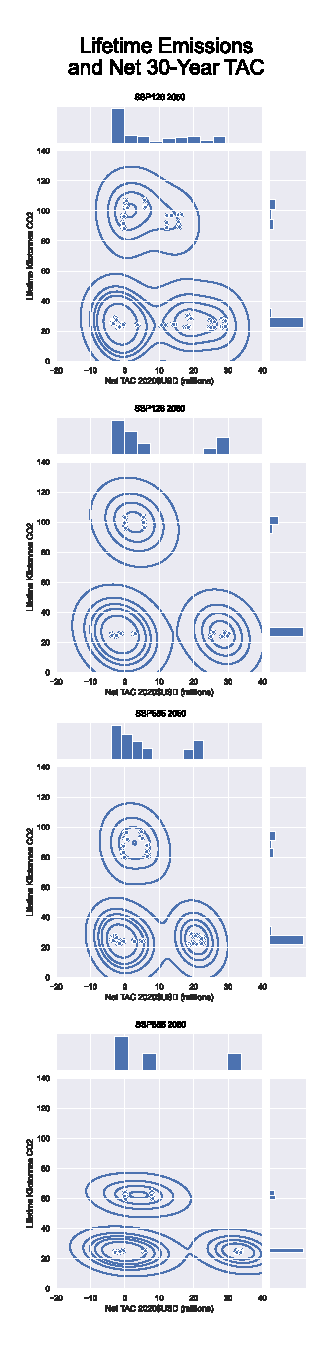
\includegraphics[scale=1.0]{figures/general_results.eps}
    \caption{General results from the iterations.}
    \label{fig:joint_plot}
\end{figure}

\subsection*{Visualizing decision making}
Marginal abatement cost and the adaptation metric were plotted to evaluate the Pareto front of each scenario. For each of the four combinations of development and climate change pathway, Figure \ref{fig:optimal_plots} highlights the best performing set of experiments. The charts are created under that assumption that only one strategy can be implemented at a time, with the topmost row containing all 255 experiments for each scenario and the following rows one less strategy implemented until the bottom most row which contains only a single strategy implemented. This presentation format allows us to view the optimal target and then evaluate how to achieve that by selecting strategy combinations in reverse, as suggested by the overlaid pathway. The lines in Figure \ref{fig:pareto-front} represent the set of optimal combinations for that particular group. In several cases no optimum set is reached due their only being one optimum. As a decision-making tool these types of graphs allow us to compare two base-metrics for economic decision making about mitigation and the effectiveness of the strategies as adaptation efforts.

\begin{figure*}[hbpt]
    \centering
    \includegraphics[scale=0.8]{figures/optimal_plots.eps}
    \caption{Plotting marginal abatement cost and the adaptation metric to serve as a canvas for pathway planning.}
    \label{fig:joint_plot}
\end{figure*}

MACCs were drawn as another form of visualising decision making. Figure \ref{fig:MACC_budget} is drawn under the assumption that planners are expecting a worst-case climate change scenario by the end of the century and have set a budget of an additional \$11,000,000 that could be invested across the development on mitigation and adaptation strategies. The drawn MACC then presents every possible combination under the development and climate change trajectory that falls below the budget. Another MACC was drawn, Figure \ref{fig:MACC_threshold} assuming an emissions reduction threshold of 80\% by 2050 under the best-case climate scenario. A third MACC was generated under the assumption that planners would be interested in decarbonizing without abandoning the district heating system, the bulk of the emissions.

To illustrate the construction of a more authentic MACC, we began with the combination of strategies that produced the best degree of adaptability under the worst-case climate change scenario at the end of the century, where the most hours outside of the comfort threshold were reduced. This strategy-set could have been any of those in Table \ref{tab:worst_case_adapt}. 


%---------------------------------------------------------------------------------------
\section*{Discussion}

\subsection*{}

%---------------------------------------------------------------------------------------
\section*{Conclusion}


%---------------------------------------------------------------------------------------
\section*{Acknowledgment}


%---------------------------------------------------------------------------------------
This document is a summary of various documents from previous Building Simulation Conferences.
%here starts the references
\bibliographystyle{BS2021}
\bibliography{references}
\newpage
\onecolumn
Please \textbf{do not} include this disclaimer in your paper.  You will be required to accept these conditions when you  submit your paper via the web site.

\begin{figure*}[ht]
\centering

\end{figure*}

\end{document}
